\subsection{MVP}
\label{MVP}
MVP (Model-View-Presenter) ist ein Design Pattern ähnlich dem MVC
(Model-View-Controller). Google beschreibt den Nutzen des MVP Patterns in der
Einbindung von Testfällen in einer GWT Anwendung. Darüber hinaus kann dieses
Pattern auch genutzt werden, um eine GWT Anwendung für verschiedene Plattformen
verfügbar zu machen. Diese Plattformen können z.B. der Browser auf mobilen
Endgeräten oder auf dem Desktop sein.
\begin{figure}[htbp]
\begin{center}
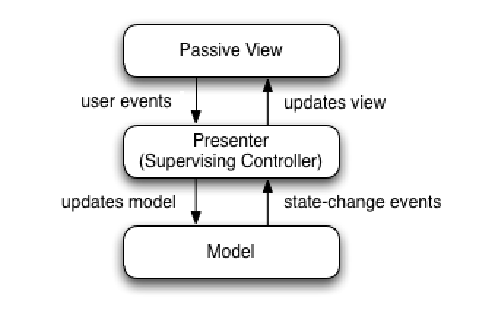
\includegraphics{./img/MVP.pdf}
\caption{Visualisierung des MVP Patterns \cite{bib:MVP1}}\label{Fig:MVP}
\end{center}
\end{figure}\\
Der Presenter übernimmt die Logik und die View ist einfach gehalten
\cite{bib:MVP2}. Dies sorgt für eine klare Trennung zwischen Model und View (vgl.
Abbildung \ref{Fig:MVP}). Bei MVC hingegen kennt die View das Model.
\cite{bib:MVCvsMVP}. Der Presenter steuert die View und übermittelt die Daten
des Model's zur View.
Daher wird der einfache Austausch von Views ermöglicht ohne das weitere
Änderungen vorgenommen werden müssen \cite{bib:MVP1}\cite{bib:MVP2}.

In der zu generierenden Anwendung soll dieses Pattern ohne ein Model
implementiert werden, da der Fokus ausschließlich auf eine GWT Frontend
Anwendung gerichtet ist. Die MVP Struktur ist dabei so umgesetzt, sodass der
Presenter als Interface in dem View Interface und konkret über die Activity
definiert wird. Die Activity regelt zusätzlich das Event Handling und die
Datenbeschaffung. Die View Implementierung beinhaltet eine
Instanz des Presenters, damit die Aktionen der View Komponenten
(bei GWT Widgets genannt) an den Presenter übergeben und dadurch an die
Activity weitergeleitet werden.
